\documentclass[11pt]{report}

% FONT %

\usepackage[utf8]{inputenc}
\usepackage[T1]{fontenc}
\usepackage[italian]{babel}
\usepackage{lmodern}

% IMMAGINI %

\usepackage{graphicx}
\usepackage{float}

% MATH % 

\usepackage{amsmath}
\usepackage{amsfonts}

% ARRAY %

\renewcommand\arraystretch{1.25}

% COLORI %

\usepackage[usenames,dvipsnames,svgnames,table]{xcolor}

\definecolor{mygreen}{rgb}{0,0.6,0}
\definecolor{mygray}{rgb}{0.5,0.5,0.5}
\definecolor{mymauve}{rgb}{0.58,0,0.82}

% LINK %

\usepackage{url}
\usepackage{breakurl}
\usepackage{hyperref}
\hypersetup{
    colorlinks=true, % false: boxed links; true: colored links
    citecolor=black,
    filecolor=black,
    linkcolor=black, % color of internal links
    urlcolor=Maroon  % color of external links
}

% CODICE %

\usepackage{framed}
\usepackage{listings}

\lstset{ %
  backgroundcolor=\color{white},   % choose the background color; you must add \usepackage{color} or \usepackage{xcolor}; should come as last argument
  basicstyle=\ttfamily,        % the size of the fonts that are used for the code
  breakatwhitespace=false,         % sets if automatic breaks should only happen at whitespace
  breaklines=true,                 % sets automatic line breaking
  captionpos=b,                    % sets the caption-position to bottom
  commentstyle=\color{mygreen},    % comment style
  extendedchars=true,              % lets you use non-ASCII characters; for 8-bits encodings only, does not work with UTF-8
  frame=single,	                   % adds a frame around the code
  keepspaces=true,                 % keeps spaces in text, useful for keeping indentation of code (possibly needs columns=flexible)
  keywordstyle=\color{blue},       % keyword style
  language=Java,                 % the language of the code
  numbers=left,                    % where to put the line-numbers; possible values are (none, left, right)
  numbersep=5pt,                   % how far the line-numbers are from the code
  numberstyle=\tiny\color{mygray}, % the style that is used for the line-numbers
  rulecolor=\color{black},         % if not set, the frame-color may be changed on line-breaks within not-black text (e.g. comments (green here))
  showspaces=false,                % show spaces everywhere adding particular underscores; it overrides 'showstringspaces'
  showstringspaces=false,          % underline spaces within strings only
  showtabs=false,                  % show tabs within strings adding particular underscores
  stepnumber=1,                    % the step between two line-numbers. If it's 1, each line will be numbered
  stringstyle=\color{mymauve},     % string literal style
  tabsize=2,	                   % sets default tabsize to 2 spaces
}

\author{Riccardo A. \\ Federico Z.}
\title{Appunti di Ingegneria del Software}

\begin{document}

\maketitle

\section*{Premesse}
Questi appunti sono stati scritti per uso personale, quindi non puntano alla formalità, né alla completezza e non sono in nessun modo da considerare una sostituzione allo studio personale del libro e delle lezioni. 
Alcuni esempi e immagini sono stati presi direttamente dalle slide del corso.

\section*{Riferimenti e fonti}
\begin{itemize}
\item Libro "Ingegneria del Software" di Ian Sommerville, decima edizione\\
\url{https://www.amazon.it/gp/product/8891902241/}
\item Libro "UML Distilled" di Martin Fowler, quarta edizione\\
\url{https://www.amazon.it/gp/product/8891907820/}
\item Slide del corso - Parte 1 \\
\url{http://www.math.unipd.it/~tullio/IS-1/2017/}
\item Slide del corso - Parte 2 \\
\url{http://www.math.unipd.it/~rcardin/sweb-2018.html}
\item Repository GitHub del documento \\
\url{https://github.com/ARDbones/SWE}
\end{itemize}

\tableofcontents
\newpage

% Progettazione
\chapter{Progettazione}

Progettare per:
\begin{itemize}
\item Dominare la complessità del prodotto ('divide-et-impera')
\item Organizzare e ripartire le responsabilità di realizzazione
\item Produrre in economia (efficienza)
\item Garantire qualità (efficacia)
\end{itemize}


L'analisi usa un approccio investigativo per capire quale è il problema.
La progettazione usa un approccio sintetico per descrivere come arrivare alla soluzione al meglio.

Problema $\to$ l'analisi approfondisce il problema $\to$ Requisiti $\to$ la progettazione sintetizza la soluzione $\to$ Soluzione

\section{La modellazione}

La modellazione è il processo che sviluppa modelli astratti di un sistema, dove ogni modello rappresenta una diversa prospettiva del sistema.
Un modello non è la rappresentazione completa del sistema, in quanto tralascia volontariamente dei dettagli per rendere più comprensibile il sistema, a meno che i modelli non vengano usati direttamente per l'implementazione, in quel caso devono essere dettagliati e completi.
Ci sono diverse prospettive secondo cui modellare:
\begin{itemize}
\item prospettiva esterna, viene modellato il contesto in cui opera il sistema
\item prospettiva di interazioni, vengono modellate le interazioni sistema-ambiente o tra i componenti del sistema
\item prospettiva strutturale, viene modellata la struttura del sistema o l'organizzazione dei dati elaborati dal sistema
\item prospettiva comportamentale, viene modellato il comportamento dinamico del sistema
\end{itemize}

%%%%%% WIP %%%%%%%%
%\subsection{Modelli contestuali}


%\subsection{Modelli di interazione}

%Diagrammi dei casi d'uso e di sequenza

%\subsection{Modelli strutturali}

%Diagrammi di classe 

%\subsection{Modelli comportamentali}


\newpage
% UML - tutti i diagrammi
\chapter{UML}
UML (\textbf{u}nified \textbf{m}odeling \textbf{l}anguage) è uno standard creato per unificare il modo di descrivere e progettare software in ambito della programmazione ad oggetti. 

\`E un linguaggio visuale che si basa su un meta-modello, un insieme di regole e vincoli per la modellazione di problemi software.
Ha una sintassi e una semantica ben definita. Uno dei vantaggi di UML è l'indipendenza dai linguaggi di programmazione.

I principali diagrammi trattati sono:
\begin{itemize}
\item diagrammi dei Casi d'Uso
\item diagrammi delle Classi
\item diagrammi dei Package
\item diagrammi di Sequenza
\item diagrammi di Attività
\end{itemize} 

\begin{figure}[H]
    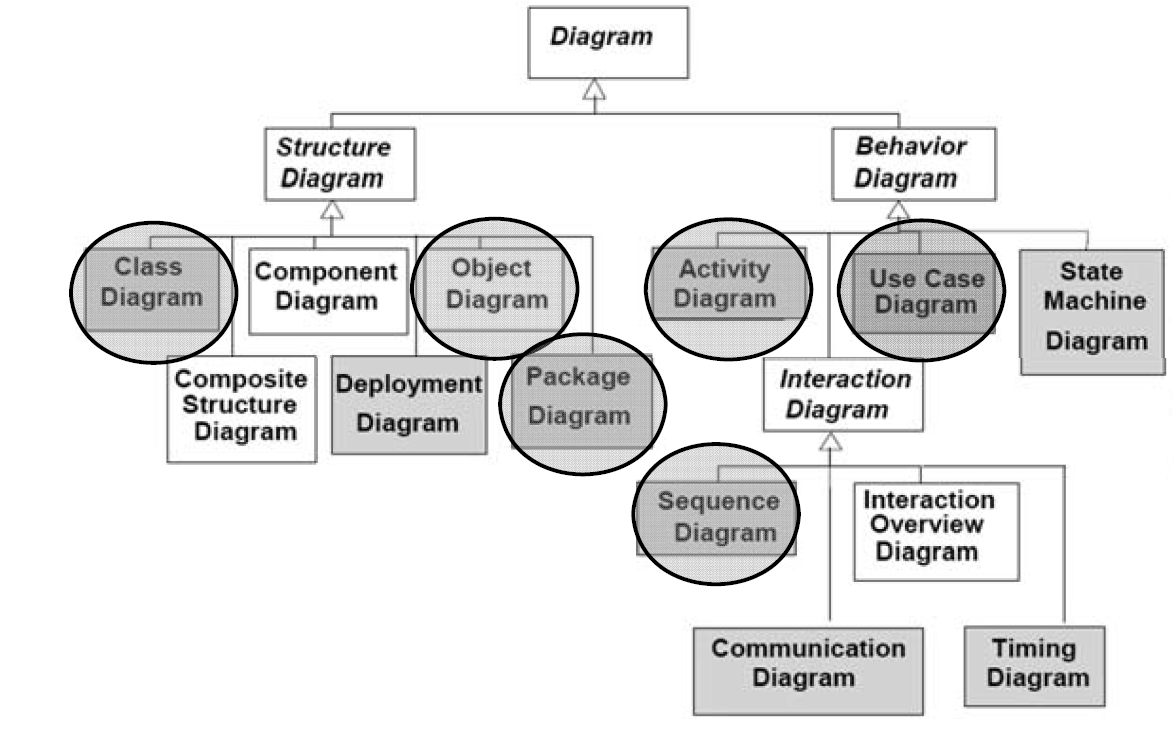
\includegraphics[width=1\textwidth]{res/img/diagrammiUML}
\end{figure}

\section{Diagrammi dei Casi d'Uso}

I diagrammi dei Casi d'Uso fanno parte dei diagrammi di comportamento. 

\subsection{I casi d'uso}
Un caso d'uso è un insieme di scenari (sequenze di azioni) che hanno in comune uno scopo finale (obiettivo) per un utente (attore),
\textit{cioè} un caso d'uso è una situazione nella quale il sistema viene utilizzato per soddisfare uno o più bisogno dell'utente.

Le funzionalità vengono descritte secondo la visione esterna, ovvero come vengono viste dall'utente, e non hanno nessun dettaglio implementativo.

I casi d'uso sono descrizioni puramente testuali, mentre i diagrammi dei casi d'uso vengono descritti con UML e rappresentano graficamente le relazioni tra attori e casi d'uso.

Un caso d'uso deve essere elementare, cioè non scomponibile in casi d'uso più semplici che abbiano ancora senso compiuto per gli attori coinvolti. 
Deve essere più grande di una singola operazione su un componente. 

Elementi di un caso d'uso:
\begin{itemize}
\item Nome + Identificatore - il nome deve essere più chiaro possibile;
\item Attori principali;
\item Attori secondari;
\item Pre-condizioni;
\item Post-condizioni; 
\item Scenario principale - la sequenza di azioni svolte dagli attori e dal sistema;
\item Scenari alternativi - eccezioni/errori e come devono essere gestiti;
\item Trigger - evento scatenante del caso d'uso.
\end{itemize}

\subsubsection{Attori}

Un attore è colui che svolge il caso d'uso per raggiungere un certo obiettivo. Può essere una persona o un altro sistema. 

Un utente può avere più ruoli (diversi attori); più utenti possono avere il medesimo ruolo (singolo attore). 

Un attore può essere collegato a più casi d'uso e un caso d'uso può avere più attori. \\
Come identificare un attore:
\begin{enumerate}
\item Identificare un entità
\item L'entità è una persona che interagisce con il sistema?
\begin{itemize}
\item[\texttt{SI}] $\to$ potrebbe essere un attore, ma si deve fare attenzione alle persone che potrebbero comunque essere parte del sistema.
\item[\texttt{NO}] $\to$ l'entità è qualcosa che si può cambiare all'interno del design del sistema?
\begin{itemize}
\item[\texttt{NO}] $\to$ probabilmente è un attore.
\item[\texttt{SI}] $\to$ l'entità non dovrebbe essere un attore, in quanto tutto ciò su cui è possibile avere il controllo, è da considerarsi parte del sistema.
\end{itemize}
\end{itemize}
\end{enumerate}

\subsection{I diagrammi}

I diagrammi dei casi d'uso sono grafi con gli attori e i casi d'uso come nodi, mentre gli archi rappresentano la comunicazione attore-caso d'uso e le relazioni tra casi d'uso, che possono essere:
\begin{itemize}
\item inclusione
\item estensione
\item generalizzazione
\end{itemize}

\begin{figure}[H]
    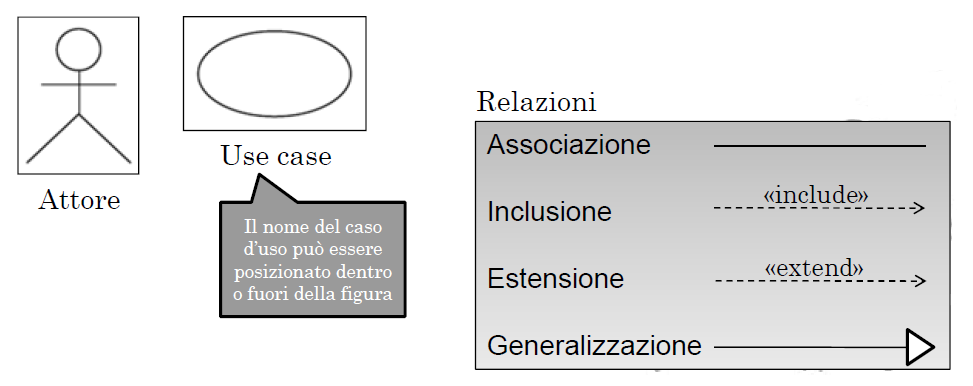
\includegraphics[width=1\textwidth]{res/img/componentiUseCaseDiagram}
    \caption{Componenti diagrammi dei Casi d'Uso (\textit{Slide E02})}
\end{figure}

\subsubsection{Inclusione}
L'inclusione viene utilizzata quando una funzionalità è comune a più casi d'uso. 
\texttt{A <<include>> B} indica che ogni istanza di A esegue B in modo incondizionato. 
A non conosce i dettagli di B, ma solo i risultati. Allo stesso modo, B non sa di essere incluso in A.

\subsubsection{Estensione}
L'estensione aumenta le funzionalità di un caso d'uso. 
\texttt{A <<extend>> B} indica che ogni istanza di A esegue B in modo condizionato, cioè l'esecuzione di B interrompe A.
Questa relazione viene spesso utilizzata per isolare in uno caso d'uso a parte la specifica di attività opzionali 
o eccezionali che potrebbero aver luogo durante l'esecuzione della funzione principale.

\subsubsection{Inclusione vs Estensione}
Entrambe le relazioni aumentano il comportamento di un caso d'uso e possono essere comuni a più casi d'uso. 
Nell'inclusione, un attore esegue sempre tutte le inclusioni, mentre nell'estensione l'attore può non eseguirle tutte.
Quindi, un'inclusione viene usata se una funzionalità si ripete in più casi d'uso; 
l'estensione se si vogliono descrivere variazioni dalla funzionalità standard. 

\subsubsection{Generalizzazione}
La generalizzazione aggiunge o modifica delle caratteristiche di base. 
Può essere usato tra attori o tra casi d'uso (più raro). 
A è generalizzazione di B se B condivide almeno le funzionalità di A.

\subsection{Individuazione Casi d'Uso}

Definizione del contesto:
\begin{enumerate}
\item Identificazione attori e responsabilità
\item Identificazione degli obiettivi da raggiungere per ciascun attore
\item Valutare attori e casi d'uso e raffinarli (divisione e accorpamento)
\item Trovare le relazioni di inclusione
\item Trovare le relazioni di estensione
\item Trovare le relazioni di generalizzazione
\end{enumerate}
Livello di dettaglio:
\begin{itemize}
\item \textbf{Kite level} - Livello molto astratto, definisce macro funzionalità
\item \textbf{Sea level} - Livello intermedio, utile nella scoperta di funzionalità nascoste
\item \textbf{Fish level} - Livello di dettaglio, da esso si individuano direttamente i requisiti del sistema
\end{itemize}

\section{Diagrammi delle Classi}
I diagrammi delle classi fanno parte dei diagrammi di struttura e si usano per rappresentare i tipi di oggetti che fanno parte di un sistema e le relazioni statiche fra i tipi. 

\subsection{Le classi}
Una classe si rappresenta:
\begin{table}[H]
\centering
\begin{tabular}{|l|}
\hline
\textbf{Nome della classe} \\
\hline
Attributo 1 \\
... \\
Attributo N \\
\hline
Operazione 1 \\
... \\
Operazione M \\
\hline
\end{tabular}
\caption{Rappresentazione di un classe}
\end{table}
Solo il nome della classe è obbligatorio, il resto è opzionale. \\
Un \textbf{attributo} è definito con:
\begin{verbatim}
Visibilità nome : tipo [molteplicità] = default {proprietà aggiuntive}
\end{verbatim}
La visibilità può essere:
\begin{itemize}
\item[\texttt{+}] public
\item[\texttt{\#}] protected
\item[\texttt{\textasciitilde}] package
\item[\texttt{-}] private
\end{itemize}
Un'\textbf{operazione} è un'azione che la classe sa eseguire ed è un servizio che può esser richiesto da ogni oggetto. Si definisce con:
\begin{verbatim}
Visibilità nome (lista-parametri) : tipo-ritorno {proprietà aggiuntive}

lista-parametri := direzione nome : tipo = default
\end{verbatim}
La visibilità si indica come per gli attributi, mentre la direzione può essere:
\begin{itemize}
\item in (default)
\item out
\item inout
\end{itemize}
Un'operazione è detta \textit{modificatore} se modifica lo stato dell'oggetto; è detta \textit{query} se non modifica lo stato. \\
\textbf{NB}: Non c'è una relazione diretta tra operazione e metodo.

Un'\textbf{associazione} è descritta da una freccia che collega due classi; a volte ha un'etichetta ed è preferibile che sia un nome piuttosto che un verbo.
Ogni associazione può avere la molteplicità che indica quanti oggetti possono far parte dell'associazione (1, 0..1, 0..*, *). 

\`E possibile aggiungere \textbf{commenti} e note in un riquadro, collegandolo con una linea tratteggiata al punto di interesse.

\subsection{Relazioni tra classi}

Due classi possono essere collegate da diversi tipi di relazione, ognuna rappresentata da un diverso tipo di freccia:
\begin{itemize}
\item dipendenza
\item associazione
\item aggregazione
\item composizione
\item generalizzazione
\end{itemize}

\begin{figure}[H]
    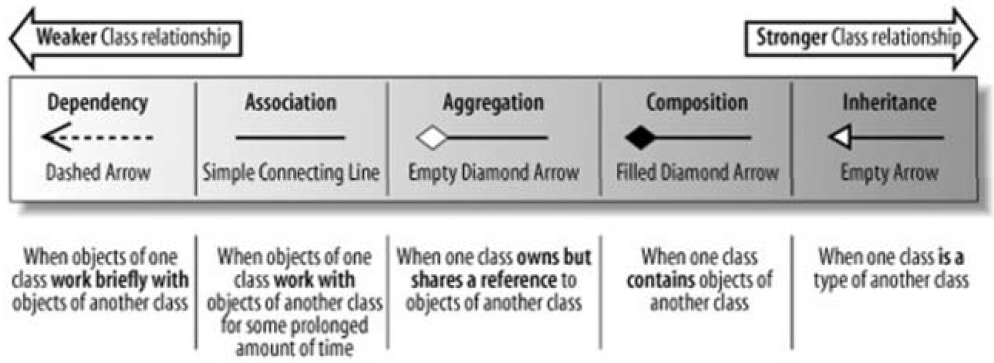
\includegraphics[width=1\textwidth]{res/img/relazioniClassi}
    \caption{Relazioni tra classi (\textit{Slide E03})}
\end{figure}

\subsubsection{Dipendenza}
Si ha una relazione di dipendenza se la modifica della definizione di un elemento può cambiare la definizione del secondo elemento. 
Maggiore è il codice condiviso tra due classi, maggiore è la dipendenza. Le dipendenze sono da minimizzare.

\textit{[Manca la lista di dipendenze UML]}

\subsubsection{Associazione}
In una normale relazione, è possibile usare classi di associazione che aggiungono attributi e operazioni alle associazioni. 
\`E una sorta di classe intermedia; per ogni coppia di oggetti, esiste una sola istanza della classe associazione. 

La classe di associazione è collegata all'associazione con una linea tratteggiata.

\subsubsection{Aggregazione}
Indica una relazione "parte di". Gli aggregati possono essere condivisi. Il \textit{diamante vuoto} della freccia è il punto di partenza della relazione.

\subsubsection{Composizione}
Come nell'aggregazione, indica una relazione "parte di", ma gli aggregati appartengono ad un solo oggetto e quest'ultimo è l'unico che può creare o distruggere le sue parti. 

Il \textit{diamante pieno} della freccia è il punto di partenza della relazione.

\subsubsection{Generalizzazione}
La generalizzazione equivale all'ereditarietà nei linguaggi di programmazione. 
A generalizza B se ogni oggetto di B è anche oggetto di A. Le proprietà ereditate non vanno ripetute nella sottoclasse.

Esistono anche la classi astratte e le interfacce. Le classi astratte hanno il nome in corsivo o \texttt{nome \{abstract\}}. La classe non è istanziabile  e le operazioni non hanno implementazioni [tutte??]. 

Le interfacce si indicano con \texttt{<<interface>> nome} nella solita forma tabellare (UML 1) o si usa un pallino con sotto il nome e le operazioni (UML 2).
Sono classi prive di implementazioni. 

\subsection{Diagrammi degli oggetti}
\`E un grafo delle singole istanze, comprensivo di associazioni e valori delle proprietà.

\begin{table}[H]
\centering
\begin{tabular}{|l|}
\hline
nome dell'istanza : nome della classe \\
\hline
nome dell'attributo = valore \\
\hline
\end{tabular}
\caption{Diagramma di un oggetto}
\end{table}

\section{Diagrammi dei Package}
I diagrammi dei Package fanno parte dei diagrammi di struttura. 


\section{Diagrammi di Sequenza}
I diagrammi di sequenza fanno parte dei diagrammi di comportamento. 


\section{Diagrammi di Attività}
I diagrammi di attività fanno parte dei diagrammi di comportamento. 


\end{document}